\documentclass{article}
\usepackage{pgfplots}
\pgfplotsset{compat=1.17}
\usepackage{tikz}
\usetikzlibrary{hobby, backgrounds}

\begin{document}

\begin{figure}
    \centering
    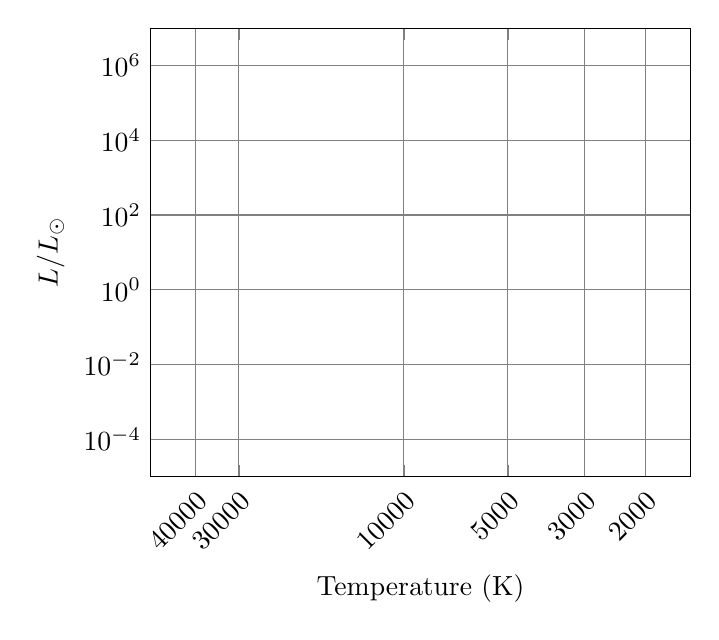
\begin{tikzpicture}
        % Logarithmic axis
        \begin{loglogaxis}[
            xlabel={Temperature (K)},
            ylabel={$L/L_\odot$},
            xmin=2000, xmax=40000,
            ymin=1e-4, ymax=1e6,
            xtick={2000, 3000, 5000, 10000, 30000, 40000},
            xticklabels={2000, 3000, 5000, 10000, 30000, 40000},
            ytick={1e-4, 1e-2, 1, 1e2, 1e4, 1e6},
            x dir=reverse, % Reverse the x-axis for Temperature
            grid=both,
            minor tick num=5,
            major grid style={black!50},
            minor grid style={gray!25},
            xticklabel style={anchor=north east, rotate=45}, % Slant the labels
            enlargelimits={0.1}, % Adds 10% extra space
            ]

            % Thinner shape by scaling the y-axis
          %  \scoped[on background layer, yscale=0.5]{ % Apply vertical scaling
           %     \path[use Hobby shortcut, closed=true, inner color=orange!80]
           %     (20000, 9e9)  
            %    .. (10000, 1e10)   
            %    .. (3000, 1e10)    
           %     .. (3000, 9e9)    
            %    .. (20000, 9e9);  
          %  }

        \end{loglogaxis}
    \end{tikzpicture}
    \caption{Hertzsprung-Russell Diagram with Thinner Supergiants Region (Vertical Scaling)}
\end{figure}

\end{document}
